\section{Sources of user activities on the Social Web}
For our research we have focused on data from two social services: \textit{YouTube} and \textit{Twitter}.
\subsection{YouTube}
\subsubsection{YouTube data}
YouTube stores various data concerning its users and content. Tables
\ref{ut_video_info} - \ref{ut_channel_info} show the types of information
available.

\begin{table}[ht]
	\begin{tabular}{|p{3cm} | l | p{4cm}|}\hline
		Information & Access & Description\\ \hline

		Title & Public API & \\
		Published & Public API & \\
		Updated & Public API & \\
		Category & Public API & \\
		Tags (keywords) & Public API & \\
		Comments & Public API & \\
		Permissons & Public API & \\
		Description & Public API & \\
		Thumbnails & Public API & Set of video's thumbnails (along with times
		when taken) \\
		Duration & Public API & \\
		Ratings & Public API & Best, worst and average rating, number of votes \\
		Viewcount & Public API & \\
		Favourite count & Public API & \\
		Number of likes & Public API & \\
		Number of dislikes & Public API & \\
		Aspect ratio & Public API & \\
		Related & Public API & \\
		Responses & Public API & \\
		Author & Public API & \\ \hline
	\end{tabular}
	\caption{Information available for a video}
\end{table}

\begin{table}[ht]
	\begin{minipage}[b]{0.5\linewidth}
	\centering
		\begin{tabular}{ | p{3cm} | l |}\hline
		Information & Access \\ \hline
		Number of results & Public API \\
		Search results & Public API \\ \hline
		\end{tabular}
		\caption{Information available for video search results}
	\end{minipage}
	\hspace{0.5cm} % no new lines here!!
	\begin{minipage}[b]{0.5\linewidth}
		\centering
		\begin{tabular}{ | p{3cm} | l |}\hline
			Information & Access\\ \hline
			Uploads & Public API \\
			Gender & Public API \\
			Location & Public API \\
			Age & Public API \\
			Contacts & Public API \\
			Username & Public API \\
			Subscriptions & Public API \\
			Inbox & Public API \\
			Favorites & Public API \\
			History & Screen scraping \\
			Likes & Screen scraping \\
			Issued authentication subtokens & Screen scraping \\ \hline
		\end{tabular}
		\caption{Information available for a user}
	\end{minipage}
\end{table}


\begin{table}[ht]
	\begin{minipage}[b]{0.5\linewidth}\centering
		\begin{tabular}{ | p{3cm} | l |}\hline
			Information & Access \\ \hline
			Created & Public API \\
			Updated & Public API \\
			Author & Public API \\
			Text & Public API \\ \hline
		\end{tabular}
		\caption{Information available for a comment}
	\end{minipage}
	\hspace{0.5cm} % no new lines here!!
	\begin{minipage}[b]{0.5\linewidth}
		\centering
		\begin{tabular}{ | p{3cm} | l |}\hline
			Information & Access \\ \hline
			Demographics & Screen scraping \\
			Referrers & Screen scraping \\
			Countries popularity & Screen scraping \\ \hline
		\end{tabular}
		\caption{Information available for a channel}
	\end{minipage}
\end{table}


\subsubsection{YouTube usage}

A statistics were performed measuring popularity of three YouTube features: favourites,
subscriptions and uploads. Over a sample of 7500 users most settled down at
relatively low level of activity. All histograms below show numbers of users
(axis y) with $x_1-x_2$ numbers of favourites/subscriptions/uploads. For all
three cases, almost all users belonged to the first histogram range -- the one
with least items. As number of items grew, the number of users decreased so
quickly, that logarithmic scale must have been used in order to make charts
readable.

\begin{figure}[ht]
  \centering
  \subfigure[Favourites]{
		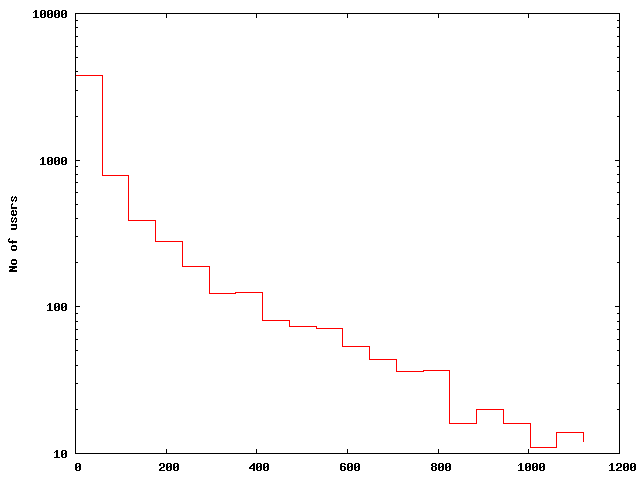
\includegraphics[scale=0.6]{images/favs.png}
		\label{fig:favs}
  }
  \subfigure[Subscriptions]{
		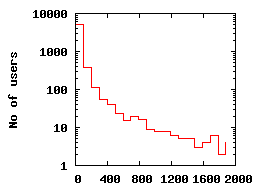
\includegraphics[scale=0.6]{images/subs.png}
		\label{fig:subs}
  }
  \subfigure[Uploads]{
		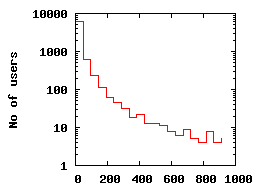
\includegraphics[scale=0.6]{images/ups.png}
		\label{fig:ups}
  }
  \label{fig:subfigureExample}
  \caption{Histograms of usage of favourites \subref{fig:favs}, subscriptions
  \subref{fig:subs} and uploads \subref{fig:ups}. The x axis represents groups of
  users having $x_1-x_2$ entities, the height of the bars indicates sizes of the
  groups.}
\end{figure}

\newpage
\subsection{Twitter}

Due to the structure of the data available on Twitter, certain approaches had to be undertaken in order to
extract information about their activities related to the media. In this section we would like to describe
available methods to achieve this as well as measurements that may be applied to the aggregated data.
We will use the word \textit{entity} to refer to known media people, shows and programmes.

\subsubsection{Available data}
\paragraph{Mentioning entities names}
Using rather trivial methods of string matching, Twitter data will be analyzed for
mentions of entities' names in tweets. Multiple occurrences of entity names in the
stream indicate interest in the entity mentioned. \\
Entities might be mentioned by:
\begin{itemize}
  \item \textit{full name} - Matching by the entities' full name.
  \item \textit{hashtag} - Matching by a Hashtag form, that is: full name stripped of all whitespace and preceded by a hash (e.g. \textit{\#TheDailyShow})
  \item \textit{twitter username} - Matching by entity's twitter username (if known) preceded by the @ character
  \item \textit{full name acronyms} - Matching acronyms built upon entity names that are longer than three words
\end{itemize}
\paragraph{Usage of preference verbs when tweeting about entities}
For extracting preference information, a vocabulary consisting of
popular preference (both positive and negative) verbs and adjectives has been used.
\paragraph{Usage of activity verbs when tweeting about entities}
Describing the activity of participating in a certain TV experience (such
as watching a show) will also need to be marked as preferential due to the
fact that Twitter users are more likely to specify what they are doing at a
particular moment)
\paragraph{Researching the structure of the most popular mentions}
By retrieving tweets containing the entities, a ranking of most popular words
appearing with the entities will be created and by extracting the most useful
ones, the vocabularies will be updated.
\paragraph{Extracting entities from structured twitter stream sources}
Some applications, such as YouTube of Boxee, can automatically generate tweets
if the user linked their Twitter account with that application. These tweets are
usually very well structured, and therefore very suitable to extract an entity, verb and/or rating from.
\paragraph{Mentioning and following entities}
An attempt will be made for relating the mentions of entities followed (for known Twitter usernames) and the mentions of those and other entities.

\subsubsection{Types of measurements available}
\begin{center}
  \begin{tabular}{ | p{4cm} | p{7cm} | } \hline
    \multicolumn{2}{|c|}{Types of measurements available} \\
    \hline
    \multirow{4}{*} {Mentioning entities}
      & Full name matching \\ \cline{2-2}
      & Matching the twitter username (if known) \\ \cline{2-2}
      & Matching name converted to a hashtag form \\
      & Matching the full name acronym \\ \cline{2-2}
    \hline
    Usage of activity verbs & Mentions using activity verbs \\
    \hline
    \multirow{3}{*}{Using preference verbs}
      & Mentions using preference verbs \\ \cline{2-2}
      & Positive preferences \\ \cline{2-2}
      & Negative preferences \\ \cline{2-2}
    \hline
    \multirow{3}{*}{Following entity}
      & Mentioning the entity by name while following \\ \cline{2-2}
      & Relation between following and actual preferences \\ \cline{2-2}
    \hline
    \multirow{3}{*}{Researching mentions}
      & Statistics of words most used with mentions \\ \cline{2-2}
      & Finding average amount of mentions-to-tweets ratio \\ \cline{2-2}
    \hline
  \end{tabular}
\end{center}

\subsubsection{Corpus used for research}
The example data to be analyzed consists of Twitter streams of over 70 users
consisting in total of about 9000 tweets. They have been selected from the followers of most popular TV channels and broadcasters available on Twitter basing on the amounts of tweets they have accumulated, the amount of their followers and the language they are tweeting in (English in this evaluation).

The most significant reason for using a preselected corpus for this research is
the Twitter API Rate Limiting which makes a wider analysis challenging.
Furthermore, a great deal of Twitter users provide completely irrelevant
information or tweet in languages not useful for this research, which also
influences the effectiveness of a limited Twitter data aggregator. Using a preselected corpus enables measuring and comparing the effectiveness of different counting methods much easier.
